\begin{center}
    \textbf{--------- Lezione 2 - 4 marzo 2021 ---------}
\end{center}
\subsection{Uso di tecniche di visione per posizione outdoor}
Dalle immagini catturate dalla macchina google (street view) possiamo estrarre dei punti di riferimento (feature points). 
La posizione da cui sono scattate le foto stradali è nota con buona precisione, quindi si riesce a conoscere la posizione dei feature points.
\\ Quando l'utente inquadra attorno a sé, si conosce più o meno la posizione, e dalle immagini dell'utente si identificato le feature che corrispondono a quelle identificate dalle immagini stradali. Poi si fa un match con i feature points della macchina google in modo tale che si possa calcolare la posizione dell'utente rispetto alla macchina (dato che so come si trova la macchina rispetto ai feature points).
Si calcola la posizione (molto precisa) e l'orientamente dell'utente. 

Una funzione simile è messa a disposizione per le librerie AR da Apple (ARKit).    

\section{Calcolo della posizione basato su segnale radio}
I dispositivi mobili al momento sono dotati di hardware per questi segnali radio:
\begin{itemize}
    \item WiFi: abbiamo un problema applicativo, con le tecnologie attuali non è possibile da programma accedere alle antenne WiFi nelle vicinanze, il SO operativo conosce le informazioni ma le API dei dispositivi iOS non consentono al programmatore di accedere. 
    \item bluetooth: dispositivi detti beacon da acquistare ed installare specificamente per il calcolo della posizione
    \item Near Field Communication (NFC)
    \item Ultra Wide-Band (UWB): ancora poco diffuso nei dispositivi mobili
\end{itemize}
RSSI indica la potenza del segnale ricevuto dal dispositivo mobile. 

Ci sono 3 diverse tecniche basate su segnale radio:
\begin{itemize}
    \item prossimità
    \item multilaterazione
    \item fingerprinting
\end{itemize}

\subsection{Posizionamento per prossimità}
Il dispositivo mobile percepisce il segnale radio inviato da un'antenna con un certo identificativo. 
Se conosciamo l'id dell'antenna e la distanza massima con la quale si può percepire il segnale da quell'antenna, allora riusciamo a scoprire la posizione di un device. 

L'accuratezza con Wifi e bluetooth è bassa mentre con NFC è alta ma il calcolo della posizione avviene solo quando l'utente avvicina il device ad un sensore NFC installato nell'ambiente.

Ci sono due limiti parlando di prossimità:
\begin{itemize}
    \item si considera una sola antenna
    \item si considera solo il fatto di percepire il segnale di quell'antenna, non si prova a stimare la distanza dall'antenna stessa
\end{itemize} 

\subsection{Multilaterazione}
Posso sapere che sono vicino ad un'antenna senza sapere la distanza oppure posso provare a stimare la distanza usando RSSI ma mi aspetto che la potenza decresca con l'aumentare della distanza.

\subsubsection{Calcolo della distanza con RSSI}
Conosciamo la potenza del segnale inviato, le caratteristiche dell'antenna, vogliamo calcolare la distanza ma abbiamo un altro fattore da prendere in considerazione che non conosciamo, il path lost factor che dipende dall'ambiente (è un fattore di attenuazione del segnale). 
\\ In ambienti aperti assume un valore di 2, in ambienti indoor tra 4 e 6 e in particolari indoor ha un valore minore di 2. 
\\ Stimando con RSSI si ottengono errori troppo grandi.
\\ Una tecnica per risolvere il problema è utilizzare un WiFi Round Trip Time.
\\ Google ha proposto una soluzione basata su RTT. 
RTT è la misura che rappresenta quanto ci mette un segnale ad andare e tornare da un'antenna. 

\subsection{Fingerprinting (o "scene analysis")}
La soluzione più adottata per risolvere i problema della multilaterazione è quella del fingerprinting.
Il valore di un RSSI in un punto è più o meno sempre quello, ma se metto più antenne, è difficile che la combinazione di questi valori si ripeta in un altro punto.

Data una posizione, il fingerprint è l’insieme di coppie $<$ID, RSSI\_ID$>$ dove ID è l’identificatore di un’antenna e RSSI\_ID il suo valore di RSSI misurato nella data posizione.

Un addetto si sposta all'interno dell'edificio segnalando al sistema la posizione corrente (es: toccando con il dito sulla mappa) e poi misura la potenza del segnale.
Questa operazione viene ripetuta in tutto l'ambiente, ad esempio ogni metro e prende le misure per tutte le antenne del fingerprint. 
\\ Il risultato prende il nome di radio map. 

La radio map contiene un insieme di coppie \textbf{$<$posizione, fingerprint$>$}, quindi \textbf{$<$posizione, [$<$ID, RSSI\_ID$>$]$>$}.

Quando un utente si trova nell'ambiente e vuole calcolare la posizione, possiamo prendere il fingerprint nella posizione corrente. 

Il modo più semplice per trovare la posizione dell'utente è: 
\begin{itemize}
    \item considerare tutti fingerprint in tutte le posizioni della radio-map
    \item calcolare il fingerprint dell'utente
    \item calcolare la distanza dal fingerprint in radio map
    \item vedere a quale campione l'utente è più vicino e assumo che quel campione sia la sua posizione
\end{itemize}


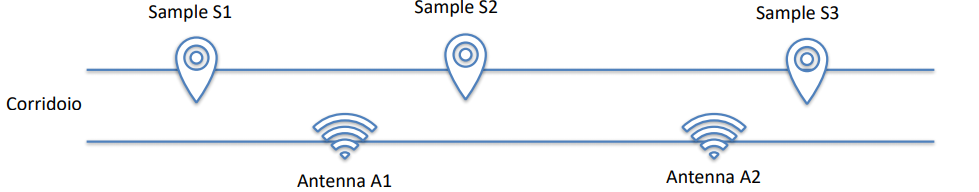
\includegraphics[width = \textwidth]{images/MobiDEV/1. posizionamento indoor/fingerprinting 1.PNG}

Ad esempio ho un corridoio con due antenne e riesco a percepirne sempre il segnale. Un incaricato misura i fingerprint in 3 posizioni campione e misura su ognuna la potenza del segnale. 
La radio map è l'insieme composto dai seguenti elementi: 
\begin{itemize}
    \item $<$S1, [$<$A1, 0,5$>$, $<$A2, 0,01$>$]$>$
    \item $<$S2, [$<$A1, 0,4$>$, $<$A2, 0,6$>$]$>$
    \item $<$S3, [$<$A1, 0,1$>$, $<$A2, 0,8$>$]$>$
\end{itemize}

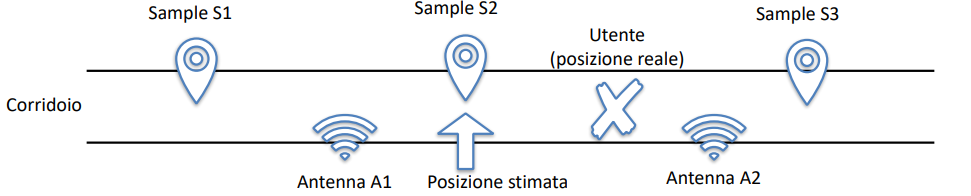
\includegraphics[width = \textwidth]{images/MobiDEV/1. posizionamento indoor/fingerprinting 2.PNG}

Il fingerprint calcolato dell'utente è [$<$A1, 0,3$>$, $<$A2, 0,7$>$].
Si procede con il calcolo delle distanze da fingerprint in radio map:
\begin{itemize}
    \item S1: $|$0,3-0,5$|$ + $|$0,7-0,01$|$ = 0,2 + 0,699 = 0,899
    \item S2: $|$0,3-0,4$|$ + $|$0,7-0,6$|$ = 0,1 + 0,1 = 0,2
    \item S3: $|$0,3-0,1$|$ + $|$0,7-0,8$|$ = 0,2 + 0,1 = 0,3
\end{itemize}
La distanza è minore rispetto ad S2 e quindi assumo che la posizione dell'utente sia quella di S2. 

Se tutto va bene trovo effettivamente il fingerprint vicino alla mia posizione. Se in fase di calibrazione ho collezionato pochi fingerprint l’errore potrebbe essere ampio, ad esempio se in un corridoio ho un fingerprint ogni 10 metri, l’errore potrebbe essere anche di 5 metri. 

Se invece, per via dei dati inesatti, scelgo un fingerprint che non è il più vicino alla mia posizione, l’errore potrebbe essere anche più grande.
\\ Per risolvere questo problema, calcolo la stessa distanza di prima ma al posto di prendere il più vicino, considero i due campioni più vicini e assumo che la posizione dell'utente sia tra quei campioni. 

Prendiamo sempre come esempio il corridoio. \\
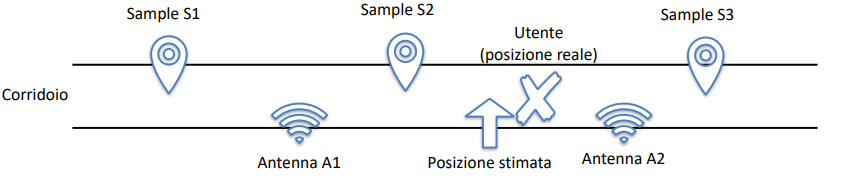
\includegraphics[width=\textwidth]{images/MobiDEV/1. posizionamento indoor/fingerprinting 3.PNG}
Si procede con il calcolo delle distanze da fingerprint in radio map, come nel caso precedente:
\begin{itemize}
    \item S1: $|$0,3-0,5$|$ + $|$0,7-0,01$|$ = 0,2 + 0,699 = 0,899
    \item S2: $|$0,3-0,4$|$ + $|$0,7-0,6$|$ = 0,1 + 0,1 = 0,2
    \item S3: $|$0,3-0,1$|$ + $|$0,7-0,8$|$ = 0,2 + 0,1 = 0,3
\end{itemize}
Successivamente stimo che la posizione dell'utente sia tra S2 ed S3 ad una distanza da S2 di 0,2 / (0,2+0,3) rispetto alla distanza totale tra S2 ed S3.

Abbiamo diversi problemi: la tecnica non è robustissima, abbiamo i dati che sono approssimativi, l'ambiente può cambiare (una porta che si apre o chiude influenza il radiomap), il numero di persone nell'ambiente influenza la radiomap, il tipo di antenna del device, l'umidità.

Bisogna avere quindi un sistema più robusto che riesca a gestire tutti questi fattori, quindi si usano tecniche probabilistiche o basate su machine learning (es: reti neurali).

C'è un altro problema, la fase di setup è molto onerosa. 
Ogni misurazione può durare anche decine di secondi. 
Ci sono vari modi per risolvere il problema:
\begin{itemize}
    \item interpolazione: l'incaricato parte da un certo punto, cammina con velocità regolare, il sistema misura la potenza del segnale e l'incaricato arriva al punto di destinazione. Il sistema sa interpolare i punti, avendo il punto di inizio e quello di fine e la velocità che è costante, l'applicazione calcola i vari fingerprint lungo il percorso
    \item robot: un sistema basato su ruote. In questo modo è più facile misurare lo spostamento. I robot esplorano l'ambiente, sappiamo quanto si spostano, in base a quanto girano le ruote
    \item crowdsourcing: non faccio fare la lettura all'incaricato ma faccio in modo che i dati vengano inseriti dagli utenti finali
\end{itemize}

\subsection{Le tecniche a confronto}

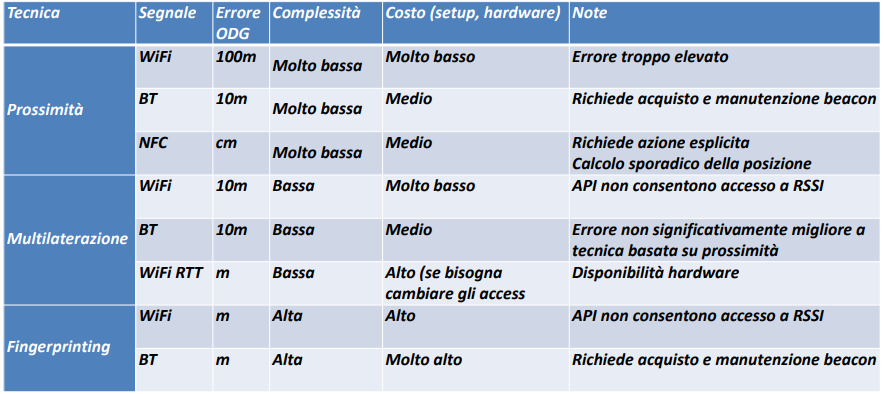
\includegraphics[width = \textwidth]{images/MobiDEV/1. posizionamento indoor/3 tecniche radio.PNG}

\begin{itemize}
    \item prossimità: hanno una minor precisione ma una maggior semplicità, hanno una costo ridotto
    \item multilaterazione: compromesso tra precisione e semplicità ma non aumentano in modo significativo la precisione
    \item fingerprinting: costo alto e complessità alta
\end{itemize}

\section{Sensori inerziali: calcolo dello spostamento}
Ci sono tecniche che permettono di calcolare la posizione come tecniche di dead reckoning utilizzate in diversi ambiti come in quello militare. Viene utilizzato un sommergibile che quando emerge, viene calcolata la posizione con GPS. Durante l'immersione, il segnale sotto una certa profondità non capisce più la posizione, per questo vengono sfruttati gli accelerometri che permettono di misurare l'accelerazione istantanea, dunque otteniamo lo spostamento. 

\textit{Si può usare in dispositivi mobili?}
\\ A bordo del sommergibile ci saranno accelerometri sicuramente più sofisticati rispetto ai telefoni. I sensori inerziali sono soggetti a meno rumore rispetto ad un telefono tenuto in mano mentre si cammina. 

Le tecniche inerziali vanno combinate con altre tecniche perché da sole non calcolano la posizione ma calcolano solo lo spostamento.
Un modo per rendere più robuste le tecniche è di combinare le tecniche inerziali con quelle visive. 

Se non conosco l'orientamento dell'utente, non serve a nulla sapere lo spostamento a meno che non usiamo filtri appositi.

\subsection{Gestione dell'errore}
Il sistema è soggetto a molte forme di errore:
\begin{itemize}
    \item potrebbe sbagliare a contare i passi o la loro lunghezza
    \item potrebbe sbagliare a calcolare la direzione
\end{itemize}
A differenza di tutte le altre tecniche, l’approssimazione nel calcolo della posizione cresce linearmente con il 
tempo. 
\\ Ad esempio ho un fix di posizione e orientamento a t=0s (errore zero). A t=2s mi aspetto un errore di posizione e orientamento contenuto: non posso aver sbagliato di tanto, in così 
poco tempo. A t=4s l’errore è dato dall’errore a t=2 più l’errore accumulato tra t=2 e t=4. Sarà sempre contenuto, ma 
generalmente maggiore dell’errore in t=2. A t=60s ho accumulato l’errore in tutti gli istanti precedenti, dunque generalmente avrò un errore ben più grande rispetto a t=2s.

Questo tipo di errore viene anche chiamato drift.

\subsection{Calcolare un passo}
In teoria è possibile calcolare quando l'utente fa un passo processando i dati di accelerometri e giroscopi. 
In termini pratici però sia iOS che Android rendono disponibile un sensore virtuale che calcola questa informazione (usando i dati di accelerometri e giroscopi), dunque è molto semplice ottenerla.
\\ Il limite di queste tecniche è che contano i passi, ma non si conosce la lunghezza del passo.
\\ Esistono diversi lavori finalizzati a calcolare la lunghezza del passo:
\begin{itemize}
    \item molti assumono che il device mobile sia solidale con il centro di massa dell'utente, come ad esempio lo smartphone legato alla cintura
    \item alcuni considerano il caso in cui il device sia tenuto in mano
    \item altri considerano che una persona faccia passi lunghi sempre uguali, in questo modo se conto i passi e so dove si sposta, posso imparare la lunghezza dei passi stessi da usare in futuro
\end{itemize}

\subsection{Tecniche visuo-inerziali}
Usando tecniche di computer vision è possibile stimare come si sta 
spostando-ruotando la camera.
Le tecniche visuo-inerziali combinano i dati dei sensori inerziali con la stima dello spostamento-rotazione ottenuta attraverso l’analisi del 
flusso video.
\\ Questo permette di ottenere una stima dello spostamento-rotazione 
più robusta rispetto al solo uso dei sensori inerziali.
\\ La tecnica è adottata dalle librerie esistenti di augmented reality.

\section{Tecniche ibride}
Combinano più soluzioni per cercare di avere una soluzione più affidabile.
\\ Un esempio di tecnica ibrida ne è il segnale radio usato in combinazione con la computer vision.
\\ Se ho due stanze identiche in piani diversi, con la tecnica computer vision risulta impossibile identificare la posizione esatta di un utente, per questo viene combinata con il segnale radio. 

Un'altra tecnica è l'utilizzo dei marcatori visivi con il calcolo della posizione. Non puoi chiedere ad un utente di spostarsi inquadrando sempre un marcatore, quindi uso i marcatori visivi. 
\\ Mentre l'utente si sposta uso le tecniche di spostamento, il problema è che dopo un po' la posizione non sarà più calcolata perfettamente, in quanto le tecniche di spostamento accumulino l'errore.
\\ Per azzerare l'errore, l'utente inquadra un marcatore visivo in modo tale che venga fatto anche un fix di posizione. 

\subsection{Tecniche ibride e calibrazione crowsourced}
In questo caso uso più tecniche di posizionamento. 
Quando una tecnica mi fornisce una posizione con buona approssimazione, ad esempio un utente inquadra un marcatore, oppure utente passa vicino ad un beacon, utilizzo questa informazione per calibrare le altre tecniche. Ad esempio tengo traccia della potenza delle antenne WiFi in quella precisa posizione.
Questo procedimento è analogo a quanto avviene in outdoor.
